% Research theme figure: Modal Decomposition and Reduced-Order Modeling
% (raw data -> modes -> pressure field). Drawn in soft colour; the website shows it
% in greyscale and reveals the colour on hover, so keep a clear light-to-dark ramp.
% Build (from this folder):
%   latex rom.tex
%   dvisvgm --no-fonts --bbox=papersize -o ../rom.svg rom.dvi
\def\pgfsysdriver{pgfsys-dvisvgm.def}
\documentclass[tikz,border=0pt]{standalone}
\usetikzlibrary{arrows.meta}
\renewcommand{\familydefault}{\sfdefault}

% --- palette: muted, light versions of common colours ----------------------
\definecolor{ink}{HTML}{1A1A1A}        % text, arrows
\definecolor{frame}{HTML}{4D4D4D}      % thin outlines
\definecolor{steel}{HTML}{245A94}      % muted blue (high pressure / strong modes)
\definecolor{sky}{HTML}{6E9FD2}        % light blue
\definecolor{mist}{HTML}{D3E3F3}       % very light blue
\definecolor{amber}{HTML}{C8702A}      % soft orange
\definecolor{sand}{HTML}{F0CFA8}       % very light orange

% --- radial shadings for the mode tiles and the pressure field -------------
\pgfdeclareradialshading{modeone}{\pgfpoint{0bp}{0bp}}{%
  color(0bp)=(steel); color(22bp)=(sky); color(34bp)=(mist); color(50bp)=(white)}
\pgfdeclareradialshading{modetwo}{\pgfpoint{0bp}{0bp}}{%
  color(0bp)=(sand); color(11bp)=(amber); color(21bp)=(sand); color(30bp)=(white); color(50bp)=(white)}
\pgfdeclareradialshading{modethree}{\pgfpoint{0bp}{0bp}}{%
  color(0bp)=(steel); color(6bp)=(mist); color(13bp)=(amber); color(21bp)=(sand);
  color(28bp)=(sky); color(34bp)=(white); color(50bp)=(white)}
\pgfdeclareradialshading{pfield}{\pgfpoint{0bp}{0bp}}{%
  color(0bp)=(steel!90!black); color(8bp)=(steel); color(20bp)=(sky); color(34bp)=(mist); color(50bp)=(mist!40!white)}

\begin{document}
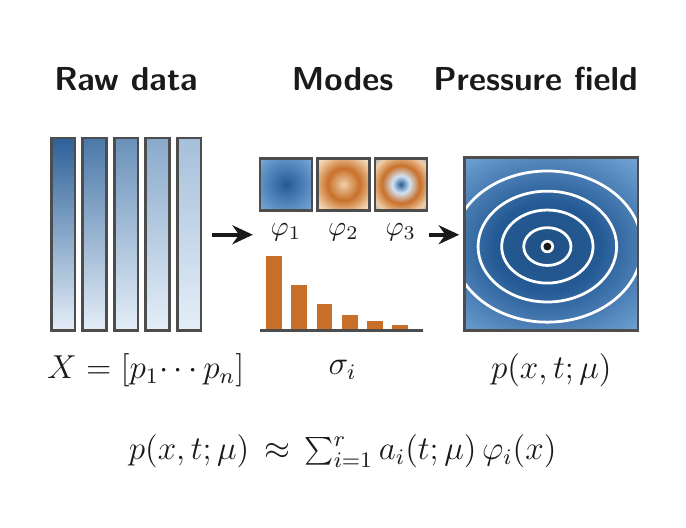
\begin{tikzpicture}[
    line width=1.6pt, >={Stealth[length=2.6mm,width=2.4mm]},
    color=ink,
    title/.style={font=\large\bfseries, text=ink},
    lab/.style={font=\large, text=ink}]
  % fixed 8 cm x 6 cm canvas
  \path[use as bounding box] (0,0) rectangle (8,6);

  % ---------------- 1) raw data: snapshot matrix X = [p_1 ... p_n] ----------------
  \node[title] at (1.25,5.35) {Raw data};
  \foreach \i/\g in {0/95,1/78,2/60,3/42,4/26} {
    \shade[top color=steel!\g!mist, bottom color=mist!60!white]
      (0.30+0.40*\i,2.15) rectangle ++(0.30,2.45);
    \draw[frame, line width=1.0pt] (0.30+0.40*\i,2.15) rectangle ++(0.30,2.45);
  }
  \node[lab] at (1.50,1.65) {$X=[p_1\!\cdots p_n]$};

  % ---------------- 2) decomposition modes and singular values ----------------
  \node[title] at (4.00,5.35) {Modes};
  \foreach \k/\s/\x in {1/modeone/2.95, 2/modetwo/3.68, 3/modethree/4.41} {
    \begin{scope}
      \clip (\x,3.68) rectangle ++(0.66,0.66);
      \shade[shading=\s] (\x+0.33,4.01) circle (0.46);
    \end{scope}
    \draw[frame, line width=1.0pt] (\x,3.68) rectangle ++(0.66,0.66);
    \node[font=\normalsize, text=ink] at (\x+0.33,3.40) {$\varphi_{\k}$};
  }
  % singular-value decay
  \foreach \i/\h in {0/0.95,1/0.58,2/0.34,3/0.20,4/0.12,5/0.07} {
    \fill[amber] (3.03+0.32*\i,2.15) rectangle ++(0.20,\h);
  }
  \draw[frame, line width=1.0pt] (2.95,2.15) -- (5.02,2.15);
  \node[lab] at (4.00,1.65) {$\sigma_i$};

  % ---------------- 3) predicted pressure field ----------------
  \node[title] at (6.45,5.35) {Pressure field};
  \begin{scope}
    \clip (5.55,2.15) rectangle (7.75,4.35);
    \shade[shading=pfield] (6.60,3.22) ellipse (2.10 and 1.75);
    \foreach \r in {0.30,0.58,0.88,1.20}
      \draw[white, line width=1.0pt] (6.60,3.22) ellipse ({\r} and {0.8*\r});
  \end{scope}
  \draw[frame, line width=1.0pt] (5.55,2.15) rectangle (7.75,4.35);
  \fill[white] (6.60,3.22) circle (0.085);
  \fill[ink] (6.60,3.22) circle (0.05);            % well
  \node[lab] at (6.65,1.65) {$p(x,t;\mu)$};

  % ---------------- arrows ----------------
  \draw[->] (2.34,3.37) -- (2.86,3.37);
  \draw[->] (5.10,3.37) -- (5.48,3.37);

  % ---------------- reconstruction ----------------
  \node[font=\large, text=ink] at (4.00,0.62)
    {$p(x,t;\mu) \,\approx\, \sum_{i=1}^{r} a_i(t;\mu)\,\varphi_i(x)$};
\end{tikzpicture}
\end{document}
